\documentclass[tikz]{standalone}

\begin{document}

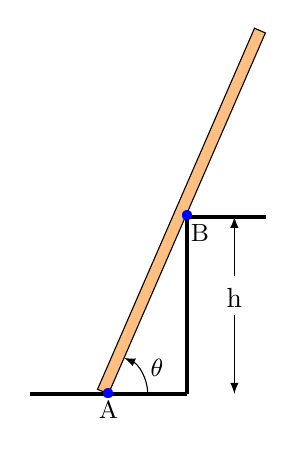
\begin{tikzpicture}
    \fill [orange!50, rotate=66.5] (0,0) rectangle (5,0.15);
    \draw[rotate=66.5] (0,0) rectangle (5,0.15);
    \draw[line width=0.5mm] (1,2.25)--(1,0);
    \draw[line width=0.5mm] (-1,0)--(1,0);
    \draw[line width=0.5mm] (1,2.25)--(2,2.25);
    \node at (0,0){\textcolor{blue}{\textbullet}};
    \node [label=below:{\small{A}}] at (0,0.15){};
    \node at (1,2.25){\textcolor{blue}{\textbullet}};
    \node [label=below right:{\small{B}}] at (0.8,2.4){};
    \draw [latex-] (1.6,2.25)--(1.6,1.5) node [label={[shift={(0,-0.65)}]h}] {};
    \draw [-latex] (1.6,1)--(1.6,0);
    \draw[-latex] (0.5,0) arc (0:66.5:0.5) node[midway,label={[shift={(0.2,-0.3)}]\small{$\theta$}}] {};
    \end{tikzpicture}

\end{document}